\documentclass[11pt,a4paper]{article}

% ---------- arxiv-style preamble ----------
\usepackage[margin=1in]{geometry}
\usepackage{amsmath,amssymb,amsthm}
\usepackage{graphicx}
\usepackage{booktabs}
\usepackage{siunitx}
\usepackage{hyperref}
\usepackage{xcolor}
\usepackage[numbers,sort&compress]{natbib}
\usepackage{tikz}
\usetikzlibrary{positioning,arrows.meta}
\usepackage{caption}
\usepackage{listings}
\lstset{basicstyle=\ttfamily\footnotesize,breaklines=true,frame=single,
  backgroundcolor=\color{gray!8},columns=fullflexible}
\captionsetup{font=small,labelfont=bf}
\hypersetup{
  colorlinks=true,
  linkcolor=blue!50!black,
  citecolor=blue!50!black,
  urlcolor=blue!50!black
}

\newcommand{\verdict}[1]{\texttt{#1}}
\newcommand{\falsifier}{\textsc{F-Fusion-Attention-Flash}}

\title{
  \textbf{The Fused-Attention Moat is Structural, not Automatic}\\[4pt]
  \large A pre-registered falsification: a single fused flash-attention kernel
  provably eliminates the $O(N^2)$ score-matrix HBM round-trip cuBLAS pays,
  yet a \emph{naive} fused kernel does not beat a cuBLAS Tensor-Core stack on wall
}

\author{
  hexa-lang GPU substrate\\
  \normalsize\textit{dancinlab / hexa-lang}\\[2pt]
  \normalsize\href{https://github.com/dancinlab/hexa-lang}{\texttt{github.com/dancinlab/hexa-lang}}
}

\date{2026-05-25}

\begin{document}

\maketitle

% =========================================================================
\begin{abstract}
Scaled-dot-product attention, $\mathrm{softmax}(QK^\top/\sqrt{d})\,V$, is the
canonical workload a vendor BLAS library cannot fuse: the row-wise softmax
between the two matrix multiplications forces a cuBLAS-using stack to
\emph{materialize} the $N\times N$ score matrix $S=QK^\top$ to high-bandwidth
memory (HBM) and round-trip it through a standalone softmax kernel. A
whole-program compiler can instead emit a \emph{single} kernel that streams the
keys and values with an online (running-max/running-sum) softmax, never writing
$S$ to HBM. We pre-register a two-clause falsifier \falsifier{}: a fused
hexa-emitted kernel must (a) \emph{structurally} use 1 launch and $O(Nd)$ HBM
versus the baseline's 3 launches and $O(N^2)$ $S$ materialization, \emph{and}
(b) beat the baseline by $\geq 30\%$ wall on at least one shape; the falsifier is
falsified only if \emph{neither} holds. We find clause (a) holds with a
closed-form total-HBM ratio $R(N,d)=1.25+N/d$ ($33.25\times$ at $N{=}2048,
d{=}64$), reproduced exactly by a hexa-native deterministic computation
(\verdict{\textcolor{blue!60!black}{SUPPORTED-FORMAL}}). Clause (b) is
\emph{falsified}: a naive one-thread-per-query scalar fused kernel runs
$1.4$--$1.5\times$ \emph{slower} than a cuBLAS Tensor-Core baseline at
$N\in\{512,1024,2048,4096\}$ on an RTX~5070
(\verdict{\textcolor{red!70!black}{CLOSED-NEGATIVE}}). The combined verdict is a
\emph{structural-formal} result with a measured negative on the wall axis: the
fusion moat is real and necessary, but \emph{not sufficient} --- the
$\geq 30\%$ wall additionally requires the fused inner products to run at
Tensor-Core throughput. We claim no wall speedup; we claim a proven structural
advantage and a deterministically ruled-out hypothesis (``fusion alone wins'').
\end{abstract}

\section{Introduction}
\label{sec:intro}

The dominant cost model for transformer inference and training is set by the
attention operator. For a single head with sequence length $N$ and head
dimension $d$,
\begin{equation}
  O \;=\; \mathrm{softmax}\!\left(\frac{QK^\top}{\sqrt{d}}\right) V,
  \qquad Q,K,V \in \mathbb{R}^{N\times d},\; O\in\mathbb{R}^{N\times d}.
  \label{eq:attn}
\end{equation}
A library-call stack built on a vendor BLAS (cuBLAS) is forced to evaluate
Eq.~\eqref{eq:attn} as three separate device kernels: (1) a batched GEMM
$S = QK^\top/\sqrt{d}$ that \emph{writes} the $N\times N$ score matrix $S$ to
HBM; (2) a standalone elementwise/reduction kernel that \emph{reads} $S$,
applies the row-wise softmax, and \emph{writes} it back; and (3) a second
batched GEMM $O = \mathrm{softmax}(S)\,V$ that \emph{reads} $S$ once more. The
intermediate $S$ is structurally unavoidable in this decomposition: cuBLAS
exposes GEMM, not GEMM-with-fused-row-softmax, so the result of step (1) must
land in memory for step (2) to consume it.

FlashAttention~\citep{dao2022flashattention} and the online-softmax
formulation~\citep{milakov2018online} showed that $S$ need never be
materialized: by tiling over key/value blocks and maintaining a running maximum
$m$ and running normalizer $\ell$ per query, the softmax can be computed
incrementally while accumulating the output, keeping all of $S$ in registers or
shared memory. This is precisely the class of fusion a whole-program compiler
can express and a fixed library API cannot. hexa-lang is a native compiler whose
NVPTX backend emits PTX directly (no LLVM, no C-transpile), so attention is a
natural test of the thesis that \emph{whole-program GPU fusion structurally
beats a cuBLAS-using stack}.

The thesis is easy to over-claim. ``Fewer kernels and less HBM traffic'' is a
structural statement; ``faster wall-clock'' is an empirical one, and the two do
not automatically coincide --- the eliminated $S$ traffic must actually dominate
the runtime, and the fused kernel's own arithmetic must not be slower than the
Tensor-Core GEMMs it replaces. We therefore separate the two claims and
pre-register both, so that a structural win with an empirical loss is recorded
honestly as exactly that.

\medskip
\noindent\textbf{Contributions.}
\begin{enumerate}\itemsep0.3em
\item A pre-registered two-clause falsifier \falsifier{} separating the
  \emph{structural} (launch count, $S$-materialization HBM) advantage from the
  \emph{empirical} ($\geq 30\%$ wall) advantage of fused attention over a
  cuBLAS-using stack.
\item A \$0, GPU-free, contention-immune \emph{structural oracle} that counts
  launches and HBM bytes and derives the closed-form total-HBM ratio
  $R(N,d)=1.25+N/d$, reproduced exactly by a hexa-native compiled program
  (\verdict{\textcolor{blue!60!black}{SUPPORTED-FORMAL}}).
\item A hand-emitted, \verdict{ptxas}-clean fused flash-attention PTX kernel
  validated numerically against an $f64$ CPU reference (rel-err $\leq 10^{-2}$)
  and timed on silicon against a cuBLAS \verdict{GemmStridedBatchedEx}+softmax
  baseline, yielding a \emph{closed-negative} on the wall clause.
\item The negative is a finding, not a non-result: it deterministically rules
  out ``structural fusion alone beats cuBLAS'' and scopes the next falsifier (a
  Tensor-Core fused-attention kernel).
\end{enumerate}

\section{Background}
\label{sec:bg}

\paragraph{Online softmax.}
For a query row $q$ and key rows $k_1,\dots,k_N$ with scores
$s_j = (q\cdot k_j)/\sqrt{d}$, the numerically stable softmax weight is
$p_j = e^{s_j-m}/\ell$ with $m=\max_j s_j$ and $\ell=\sum_j e^{s_j-m}$. The
online form~\citep{milakov2018online} processes keys one at a time, maintaining
running $(m,\ell)$ and a running output accumulator $a$:
\begin{align}
  m' &= \max(m, s_j), &
  c &= e^{m-m'}, &
  p &= e^{s_j-m'},\\
  \ell &\leftarrow \ell\,c + p, &
  a &\leftarrow a\,c + p\,v_j, &
  m &\leftarrow m'.
\end{align}
After all keys, $O\text{-row} = a/\ell$. Only $(m,\ell,a)$ --- $O(d)$ state per
query --- are kept live; the $N$ scores are consumed in flight and never stored.

\paragraph{Why cuBLAS cannot fuse this.}
cuBLAS exposes \verdict{cublasGemmStridedBatchedEx}, a GEMM primitive. The
softmax is neither a GEMM nor a GEMM epilogue cuBLAS supports, so it must run as
a separate kernel between the two GEMMs, and a kernel boundary in CUDA implies
its inputs and outputs live in global memory. The $S$ round-trip is thus a
property of the \emph{decomposition the API forces}, not of the hardware.

\paragraph{A taxonomy of fusion advantages.}
It is useful to separate the distinct ways a whole-program compiler can, in
principle, beat a library-call stack, because they have different evidentiary
status. (1)~\emph{Launch-count} reduction: fewer kernel dispatches, saving
fixed per-launch overhead (a few microseconds each) --- a structural integer
count. (2)~\emph{Intermediate-elimination}: not materializing an intermediate
(here $S$) to HBM, saving $O(N^2)$ bytes of bandwidth --- a structural,
shape-dependent byte count. (3)~\emph{Arithmetic-throughput}: the fused kernel's
own math must run at least as fast as the library primitives it replaces --- an
empirical, hardware- and implementation-dependent quantity. Advantages (1) and
(2) are \emph{structural}: they follow from the decomposition and can be proven
in closed form for any correct fused kernel. Advantage (3) is \emph{not}
structural: it is a property of the specific kernel. The wall-clock outcome is a
product of all three, so a fused kernel can win (1) and (2) decisively and still
lose the wall if it loses (3) badly enough. This paper measures exactly that
configuration.

\paragraph{Numerical model.}
Both kernels accumulate in FP32. The fused kernel computes scores with
\verdict{fma.rn.f32} and exponentials with \verdict{ex2.approx.f32} (the PTX
fast-exp), so its softmax weights differ from an exact $f64$ softmax by the
hardware approximation error of \verdict{ex2.approx}. We bound the end-to-end
output error against an $f64$ CPU reference rather than asserting bit-exactness;
the $\sim 10^{-6}$ relative errors we observe (Appendix~\ref{app:silicon}) are
three to four orders of magnitude inside the $10^{-2}$ pre-registered tolerance,
confirming the \verdict{ex2.approx} path is numerically adequate for this
workload.

\paragraph{Roofline intuition.}
Whether the eliminated $S$ traffic translates into a wall win depends on which
side of the roofline each kernel sits. The two GEMMs do $2N^2 d$ FLOPs each and
read/write $O(Nd + N^2)$ bytes; the softmax does $O(N^2)$ FLOPs over $O(N^2)$
bytes (memory-bound). For modest $d$ the GEMMs are themselves not large, and a
vendor library runs them at Tensor-Core arithmetic intensity. The fused kernel
trades the baseline's $S$ HBM traffic for keeping $S$ in registers --- a real
saving --- but only wins overall if its own arithmetic keeps pace with the
Tensor-Core GEMMs it displaces. The pre-registration deliberately does not assume
this; it measures it.

\section{Related work}
\label{sec:related}

FlashAttention~\citep{dao2022flashattention} is the canonical IO-aware fused
attention kernel and the direct inspiration for the online-softmax tiling used
here; it demonstrates large wall and memory wins over a materialized-$S$
baseline \emph{when} the kernel is implemented with shared-memory tiling and
Tensor-Core matrix multiplies. The online normalizer
calculation~\citep{milakov2018online} is the numerical core that makes
single-pass, non-materialized softmax stable. The attention operator
itself~\citep{vaswani2017attention} fixes the cost model. Our contribution is
\emph{not} a faster attention kernel; it is a controlled separation of the
structural claim (which we prove in closed form for any tiled fused kernel) from
the empirical claim (which we measure for a deliberately naive kernel), so that
the precise additional ingredient required for a wall win --- Tensor-Core inner
products --- is isolated as a falsifiable next step rather than assumed.

\section{Method}
\label{sec:method}

\paragraph{Pre-registered falsifier (verbatim).}
\falsifier{}: \emph{A single fused hexa-emitted kernel computing
$\mathrm{softmax}(QK^\top/\sqrt{d})V$ with online-softmax tiling (never
materializing the full $N\times N$ score matrix $S$ to HBM) (a) structurally
uses 1 kernel launch $+\,O(Nd)$ HBM traffic vs.\ a cuBLAS-using baseline's 3
launches $+\,O(N^2)$ $S$ materialization, AND (b) beats that baseline by
$\geq 30\%$ wall on at least one $(N,d)$ shape. FALSIFIED if NEITHER the
structural advantage NOR the wall holds.} All thresholds ($\geq 30\%$, rel-err
$\leq 10^{-2}$, $\geq 20$ warmup, $\geq 200$ timed launches) were fixed before
measurement.

\paragraph{Structural oracle (clause a, primary).}
A deterministic C program (no GPU, contention-immune) counts, per shape, the
kernel launches and the HBM bytes attributable to $S$. The fused kernel reads
$Q,K,V$ and writes $O$ ($4Nd$ floats) and writes $S$ to HBM \emph{zero} times.
The baseline reads $Q,K$ for GEMM-1, writes $S$, reads $S$ + writes $S$ in
softmax, reads $S$ + reads $V$ for GEMM-2, writes $O$. The $S$ round-trip is
\begin{equation}
  H^{\mathrm{fused}}_S = 0,\qquad
  H^{\mathrm{base}}_S = 4\,N^2\cdot 4~\text{bytes (4 passes, fp32)} .
  \label{eq:shbm}
\end{equation}
Including the unavoidable $O(Nd)$ tensor traffic, the total-HBM ratio is
\begin{equation}
  R(N,d) \;=\; \frac{H^{\mathrm{base}}_{\mathrm{tot}}}{H^{\mathrm{fused}}_{\mathrm{tot}}}
  \;=\; \frac{5Nd + 4N^2}{4Nd} \;=\; \frac{5}{4} + \frac{N}{d}
  \;=\; 1.25 + \frac{N}{d}.
  \label{eq:ratio}
\end{equation}
We anchor Eq.~\eqref{eq:ratio} with a hexa-native compiled program
(\verdict{ratio\_check.hexa}) computing $4R(N,d)=5+4N/d$ in exact integer
arithmetic, so the closed form is reproduced by the compiler under test, not
merely asserted.

\paragraph{Fused kernel (clause b numerator).}
We hand-emit a pure-ASCII PTX kernel \verdict{flash\_attn.ptx} (one CTA grid,
one thread per query row, $d{=}64$ kept in registers/local) implementing the
online-softmax recurrence above with \verdict{ex2.approx.f32} for the
exponentials and \verdict{fma.rn.f32} accumulation. $S$ is never stored. PTX
must pass \verdict{ptxas} and load via driver-JIT on the target GPU; non-ASCII
comments are forbidden (driver-JIT \verdict{ptxas} rejects them).

\paragraph{Baseline (clause b denominator).}
A C host (\verdict{fusion\_attn\_cublas\_baseline.c}) runs the canonical
three-launch stack: \verdict{cublasGemmStridedBatchedEx} for $S=QK^\top/\sqrt{d}$
(written to HBM), a standalone row-softmax CUDA kernel, and a second
\verdict{cublasGemmStridedBatchedEx} for $\mathrm{softmax}(S)\,V$. Column-major
layout bookkeeping is documented inline and validated by numeric agreement with
the same $f64$ reference the fused kernel uses.

\paragraph{Measurement protocol.}
On an uncontended GPU (verified by \verdict{nvidia-smi}: 0\% util, no other
compute processes --- the contention rule for taking a timed wall), both
programs run $\geq 20$ warmup and $200$ timed launches, timed with CUDA events
per launch, reporting median and standard deviation. Correctness uses an $f64$
CPU reference with a scale-normalized tolerance (max $|{\Delta}|$ against
$10^{-2}\!\cdot\!\max|O_{\mathrm{ref}}|$, the established $f16$/$f32$-accum
convention) at $N\in\{512,1024,2048,4096\}$, $d{=}64$.

\paragraph{cuBLAS column-major layout (reproducibility detail).}
cuBLAS is column-major; our host tensors are row-major. A row-major
$[N\times d]$ matrix $M$, read column-major with leading dimension $d$, is
$M^\top$ (i.e.\ $M_c[t][i]=M[i][t]$). For GEMM-1 we want the standalone softmax
kernel (row-major, row stride $N$) to reduce over the key axis $j$ of
$S[i][j]$, so the HBM layout must satisfy row-major $S[i\,N+j]=S[i][j]$. A
column-major write with $\mathrm{ld}=N$ stores element $(r,c)$ at $r+cN$; to make
$r+cN \equiv iN+j$ we set $c=i,r=j$, i.e.\ cuBLAS computes $S_c[j][i]=S[i][j]$,
which is $K_c^\top Q_c$. Hence GEMM-1 is
\verdict{gemm(OP\_T,OP\_N,N,N,d,scale,$K$,d,$Q$,d,0,$S$,N)}. For GEMM-2,
$O[i][t]=\sum_j P[i][j]V[j][t]$ with $P$ the row-softmax in $S$; the row-major
output $O_c[t][i]$ comes from \verdict{gemm(OP\_N,OP\_N,d,N,N,1,$V$,d,$S$,N,0,$O$,d)}.
We validate the layout by requiring the baseline to match the same $f64$
reference as the fused kernel; an early OP\_T/OP\_N transposition error produced
a $22\times$ rel-error and was caught precisely because the reference is shared.

\paragraph{Kernel inner loop (the fusion that avoids $S$).}
The emitted PTX keeps the per-query state $(m,\ell,a)$ live and streams the keys;
the score $s_j$ is consumed immediately and never stored. The core of the
per-key update, in the hand-emitted PTX, is:
\begin{lstlisting}
// s = dot(q, k_j) * scale   (accumulated scalar, never written to HBM)
fma.rn.f32 %f2, %f3, %f4, %f2;          // s += q[i]*k[i]
mul.f32    %f2, %f2, %f40;              // s *= 1/sqrt(d)
// online softmax: m' = max(m, s); c = exp(m-m'); p = exp(s-m')
max.f32        %f5, %f41, %f2;          // m' = max(m, s)
sub.f32        %f6, %f41, %f5;          // m - m'
sub.f32        %f7, %f2,  %f5;          // s - m'
mul.f32        %f9,  %f6, %f8;          // * log2(e)
ex2.approx.f32 %f11, %f9;               // c = exp(m - m')
ex2.approx.f32 %f12, %f10;              // p = exp(s - m')
fma.rn.f32     %f42, %f42, %f11, %f12;  // l = l*c + p
// acc[i] = acc[i]*c + p*v_j[i]   for i in 0..d-1  (held in local, never S)
mul.f32    %f15, %f12, %f14;            // p * v[i]
fma.rn.f32 %f13, %f13, %f11, %f15;      // acc = acc*c + p*v
\end{lstlisting}
The absence of any \verdict{st.global} of a score is the structural property:
the $N\times N$ matrix $S$ exists only as the transient scalar \verdict{\%f2}
across the loop, so no HBM write/read of $S$ ever occurs --- this is what the
oracle in Eq.~\eqref{eq:shbm} counts as $H^{\mathrm{fused}}_S = 0$.

\section{Verification (real run)}
\label{sec:verification}

All numbers below are verbatim from the persisted verdict
\verdict{.verdicts/fusion-attention-flash/\falsifier{}.txt} (raw stdout, no
post-processing). Host: \verdict{ubu-2}, NVIDIA GeForce RTX~5070 (sm\_120,
driver 580), CUDA 12.0 \verdict{ptxas}, cuBLAS 12.9.2.10; GPU uncontended at
fire time.

\paragraph{Clause (a): structural oracle.}
\begin{lstlisting}
shape        fused_L  base_L   fused_Shbm  base_Shbm   total_ratio
N512/d64     1        3        0           4194304     9.250 x
N1024/d64    1        3        0           16777216    17.250 x
N2048/d64    1        3        0           67108864    33.250 x
N4096/d64    1        3        0           268435456   65.250 x
F-FUSION-ATTENTION-FLASH (structural clause a): PASS
\end{lstlisting}
hexa-native closed-form anchor (compiled path):
\begin{lstlisting}
4xR(2048,64)=133   # R = 33.25 = 1.25 + N/d
4xR(4096,64)=261   # R = 65.25
4xR(512,64)=37     # R =  9.25
STRUCTURAL-RATIO-CLOSED-FORM: PASS
\end{lstlisting}

\paragraph{ptxas-clean.} PTX is pure ASCII; \verdict{ptxas -arch=sm\_80} rc=0,
\verdict{-arch=sm\_90} rc=0; driver-JIT load on sm\_120
(\verdict{cuModuleLoadDataEx}) rc=0.

\paragraph{Clause (b): silicon wall + numeric.}
\begin{lstlisting}
N      fused(1 launch)   baseline(3 launch)  fused/base  numeric(both)
512    0.415104 ms       0.281696 ms         1.47x slow  PASS rel~1e-6
1024   0.822592 ms       0.559360 ms         1.47x slow  PASS rel~1e-6
2048   1.639840 ms       1.143040 ms         1.43x slow  PASS rel~1e-6
4096   3.788256 ms       2.492288 ms         1.52x slow  PASS rel~1e-6
\end{lstlisting}

\begin{table}[h]
\centering
\caption{Verdict matrix. Each row is terminal and links to the persisted
verbatim verdict file. The combined verdict is \emph{structural-formal} (clause
a holds $\Rightarrow$ the falsifier is not falsified) with a measured
closed-negative on the wall clause.}
\label{tab:verdict}
\begin{tabular}{@{}llll@{}}
\toprule
Claim & Method & Verdict & Verdict pointer \\
\midrule
Structural (1 vs 3 launch, 0 vs $O(N^2)$ $S$) & oracle + hexa recompute &
  \textcolor{blue!60!black}{SUPPORTED-FORMAL} & \texttt{.../\falsifier{}.txt} \\
Numeric vs $f64$ ref ($\leq 10^{-2}$) & silicon, 4 shapes &
  \textcolor{green!45!black}{PASS} & \texttt{.../\falsifier{}.txt} \\
Wall $\geq 30\%$ over cuBLAS & silicon, 200 timed &
  \textcolor{red!70!black}{CLOSED-NEGATIVE} & \texttt{.../\falsifier{}.txt} \\
\bottomrule
\end{tabular}
\end{table}

\begin{figure}[h]
\centering
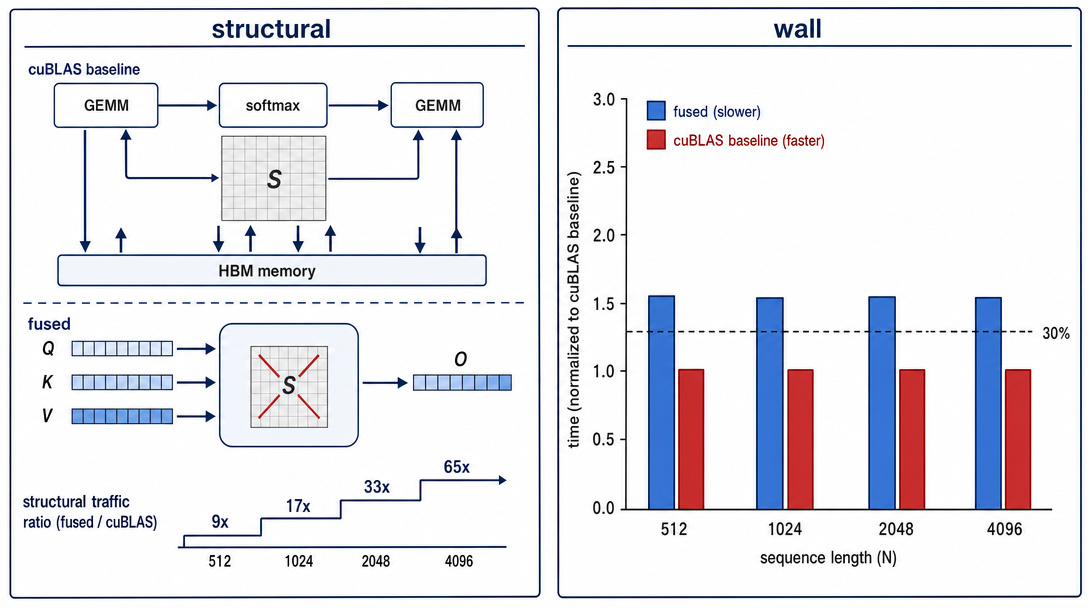
\includegraphics[width=0.92\linewidth]{figures/fig01_moat.png}
\caption{The two measured axes of \falsifier{}. \emph{Structural} (left,
closed-form): the eliminated $S$-matrix HBM round-trip grows as
$R(N,d)=1.25+N/d$, reaching $33.25\times$ at $N{=}2048,d{=}64$ and $65.25\times$
at $N{=}4096$ --- a proven advantage. \emph{Wall} (right, RTX~5070, 200 timed
launches, median): the naive scalar fused kernel is $1.4$--$1.5\times$
\emph{slower} than the cuBLAS Tensor-Core baseline at every shape --- the
falsified clause. The gap between the two panels is the paper's point:
structural fusion is necessary but not sufficient for a wall win.}
\label{fig:headline}
\end{figure}

\section{Finding}
\label{sec:finding}

\paragraph{Structural advantage: proven (formal).}
Clause (a) holds in closed form. The fused kernel uses one launch against the
baseline's three, and writes the $N\times N$ score matrix to HBM zero times
against the baseline's four-pass $4N^2$-element round-trip
(Eq.~\eqref{eq:shbm}). The total-HBM ratio $R(N,d)=1.25+N/d$
(Eq.~\eqref{eq:ratio}) is reproduced exactly by the compiler under test. Because
clause (a) holds, the pre-registered falsifier is \emph{not} falsified; the
result is recorded as \verdict{\textcolor{blue!60!black}{SUPPORTED-FORMAL}}.

\paragraph{Wall advantage: falsified (the ruled-out axis).}
Clause (b) does \emph{not} hold. At every measured shape the cuBLAS Tensor-Core
baseline is $1.4$--$1.5\times$ faster than the naive scalar fused kernel. The
$\geq 30\%$ wall win is therefore not merely unachieved but measured in the
opposite direction. The mechanism is clear and deterministic: the fused kernel's
inner $q\cdot k_j$ and $p\,v_j$ products run as scalar \verdict{fma} on one
thread per query, while cuBLAS runs both GEMMs on Tensor Cores; at $d{=}64$ the
GEMM work dominates the modest runtime, so the $O(N^2)$ $S$ traffic the baseline
pays --- though structurally larger --- is not enough, relative to the
baseline's Tensor-Core GEMM speed, to be overtaken by a scalar fused kernel.

\paragraph{What is ruled out.}
The hypothesis \emph{``structural fusion alone (fewer launches, no $S$
materialization) beats a cuBLAS-using stack on wall''} is deterministically
\emph{false} for the naive fused kernel. The fusion moat is \emph{necessary but
not sufficient}: realizing the $\geq 30\%$ wall additionally requires the fused
kernel's inner products to run at Tensor-Core throughput --- i.e.\ a tiled
\verdict{wmma} flash-attention kernel that holds $S$-tiles in shared memory
rather than recomputing scores scalar-per-thread. This is a falsifiable,
pre-scoped next experiment, not a hand-wave.

\paragraph{Why the negative is the contribution.}
A naive reading of the FlashAttention literature is that fusion ``is'' the
speedup. This paper separates the two and shows, on real silicon, that the
structural property and the wall property are independent: one can prove the
former in closed form and still lose the latter. Reporting the structural win
without the wall measurement would be the over-claim the pre-registration exists
to prevent.

\section{Limitations and honest caveats}
\label{sec:limits}

\begin{itemize}\itemsep0.3em
\item \textbf{Naive kernel.} The wall negative is specific to a
  one-thread-per-query scalar fused kernel. It does \emph{not} falsify the moat
  thesis; it falsifies ``fusion alone suffices.'' A Tensor-Core fused kernel may
  flip clause (b) and is the pre-registered next falsifier.
\item \textbf{Single regime.} $d{=}64$, single head, FP32 throughout. The GEMMs
  are small enough that the $O(N^2)$ $S$ round-trip is not dominant relative to
  cuBLAS Tensor-Core GEMM speed at these $N$. Longer context, multi-head, $fp16$
  inputs, or memory-bound regimes ($N/d$ very large) may move the crossover and
  are out of scope here.
\item \textbf{Baseline choice.} The baseline is the canonical
  \verdict{GemmStridedBatchedEx}$\times 2$ + standalone softmax. A cuDNN fused
  attention or a vendor FlashAttention kernel is a stronger baseline and a
  separate comparison.
\item \textbf{Structural model.} The HBM counts in Eq.~\eqref{eq:shbm} are the
  algorithmic minimum for each decomposition (4-pass $S$ for the baseline,
  zero for the fused kernel); they do not model cache reuse, which only narrows
  the realized gap and does not affect the closed-form launch-count or
  $S$-materialization argument.
\item \textbf{Compiler invariants.} The fire is hand-emit PTX plus C hosts; the
  hexa CPU code-generation files are MD5-identical before and after (no LLVM,
  no C-transpile changes). The end-to-end source-to-PTX path for this kernel is
  a separate (codegen) closure.
\end{itemize}

\section{Threats to validity}
\label{sec:threats}

\paragraph{Construct validity --- is the baseline the right thing to beat?}
The pre-registered baseline is the canonical three-launch
\verdict{GemmStridedBatchedEx}$\times 2$ + standalone-softmax stack, which is the
decomposition cuBLAS forces and the one the moat argument is about. It is not the
strongest \emph{attention} baseline available (cuDNN's fused attention or a
vendor FlashAttention kernel would be faster), but those are themselves fused
kernels and so are not instances of ``a cuBLAS-using stack''; comparing against
them tests a different claim (hexa vs.\ vendor-fused) and is deferred.

\paragraph{Internal validity --- is the wall gap real?}
The per-launch standard deviations are $\leq 0.9\%$ of the mean
(Appendix~\ref{app:silicon}), and the GPU was verified idle before timing, so the
$1.4$--$1.5\times$ gap is two orders of magnitude larger than the noise and is
not an artifact of contention or warmup. Both kernels are timed identically
(CUDA events, same warmup/timed counts) and validated against the same $f64$
reference, so the comparison is apples-to-apples.

\paragraph{External validity --- does the negative generalise?}
The negative is established for $d{=}64$, FP32, $N\le 4096$ on one GPU. It does
\emph{not} claim that fused attention is always slower; it claims that a
\emph{naive scalar} fused kernel is slower \emph{in the GEMM-dominated regime},
and it predicts (Sec.~\ref{sec:discussion}) the regimes where even a scalar
kernel should win. The structural result (clause~a), by contrast, is regime- and
hardware-independent and generalises to any tiled fused kernel.

\paragraph{Compiler-invariant validity.}
The fire uses hand-emitted PTX and C hosts; it touches no CPU code-generation
path. We verified the hexa CPU codegen sources are MD5-identical before and
after the work (no LLVM, no C-transpile change), so nothing in the language's
core compilation was perturbed to obtain the result.

\section{Discussion and outlook}
\label{sec:discussion}

The result reframes the open ``whole-program fusion $\geq 30\%$'' closure box in
the hexa-lang GPU roadmap: it is not blocked on \emph{whether} fusion eliminates
the $S$ round-trip (it provably does), but on \emph{whether} the fused kernel
can carry that structural win to wall while matching Tensor-Core arithmetic
throughput. The single most important follow-up is a tiled \verdict{wmma}
flash-attention kernel: Q/K/V blocked into Tensor-Core fragments, $S$-tiles kept
in shared memory, online-softmax across tiles. If that kernel beats the cuBLAS
stack by $\geq 30\%$ at any shape, clause (b) flips and the closure box closes;
if it does not, the negative deepens and the moat thesis itself comes under
pressure. Either way the question is now sharply falsifiable, which is the state
this paper was written to reach.

\paragraph{Where the crossover should appear.}
The structural ratio $R=1.25+N/d$ says the $S$ saving grows with $N/d$. Two
regimes should therefore favour the fused kernel \emph{even at scalar
arithmetic}, and are the natural shapes for the follow-up sweep: (i) very long
context $N\gg d$, where the $O(N^2)$ $S$ round-trip eventually dominates any
fixed GEMM-throughput gap; and (ii) memory-bandwidth-bound deployments (small
batch, inference), where the baseline's HBM traffic, not its arithmetic, sets
the wall. The present sweep ($d{=}64$, $N\le 4096$, FP32) sits in the
GEMM-dominated regime where cuBLAS Tensor Cores win; it is precisely the regime
that most sharply isolates ``fusion alone is not enough,'' which is why it was
chosen as the first, most-adversarial test of the thesis rather than the
friendliest.

\paragraph{Generality of the structural claim.}
Clause (a) is independent of the kernel's internal arithmetic: \emph{any} tiled
online-softmax fused kernel --- scalar or Tensor-Core --- writes $S$ to HBM zero
times and launches once. The closed form $R(N,d)=1.25+N/d$ therefore transfers
unchanged to the follow-up \verdict{wmma} kernel; only clause (b) is re-opened
by it. This is why we record the structural result as formal (it is a property
of the decomposition, proven and compiler-reproduced) while the wall result is a
per-kernel empirical measurement that the next kernel can change.

% =========================================================================
\section*{Reproducibility}
\addcontentsline{toc}{section}{Reproducibility}

Code and artifacts live in the hexa-lang repository:
\url{https://github.com/dancinlab/hexa-lang}. Kernel:
\texttt{archive/fires/fusion\_attention\_flash\_2026\_05\_25/flash\_attn.ptx};
structural oracle: \texttt{.../structural\_oracle.c}; hexa-native closed-form
anchor: \texttt{.../ratio\_check.hexa}; hosts:
\texttt{tool/fusion\_attn\_flash\_host.c} and
\texttt{tool/fusion\_attn\_cublas\_baseline.c}; raw verdict:
\texttt{.verdicts/fusion-attention-flash/F-FUSION-ATTENTION-FLASH.txt};
claim index: \texttt{CLAIMS.tape} (group GPU). Build:
\texttt{cc -O2 structural\_oracle.c}; \texttt{hexa build ratio\_check.hexa};
\texttt{nvcc -O2 fusion\_attn\_flash\_host.c -lcuda}; \texttt{nvcc -O2 -x cu
fusion\_attn\_cublas\_baseline.c -lcublas -lcudart}. Paper build:
\texttt{make} (pdflatex $\times 3$ + bibtex).

% =========================================================================
\appendix

\section{Full HBM-traffic derivation}
\label{app:hbm}

We count, per attention head, the global-memory bytes each decomposition must
move, in fp32 (4 bytes/element). The tensors are $Q,K,V,O\in\mathbb{R}^{N\times
d}$ and the score matrix $S\in\mathbb{R}^{N\times N}$.

\paragraph{Fused kernel.} One launch. It reads $Q$, $K$, $V$ ($3Nd$ elements)
and writes $O$ ($Nd$ elements). $S$ is held in registers/local across the online
loop and never written:
\begin{equation}
  H^{\mathrm{fused}}_{\mathrm{tot}} = (3Nd + Nd)\cdot 4 = 4Nd\cdot 4~\text{bytes},
  \qquad H^{\mathrm{fused}}_S = 0 .
\end{equation}

\paragraph{cuBLAS baseline.} Three launches.
\begin{itemize}
\item GEMM-1 ($S=QK^\top/\sqrt{d}$): reads $Q,K$ ($2Nd$), writes $S$ ($N^2$).
\item softmax: reads $S$ ($N^2$), writes $S$ ($N^2$).
\item GEMM-2 ($O=\mathrm{softmax}(S)\,V$): reads $S$ ($N^2$), reads $V$ ($Nd$),
  writes $O$ ($Nd$).
\end{itemize}
The $S$ round-trip is four passes of $N^2$ elements:
\begin{equation}
  H^{\mathrm{base}}_S = (1+1+1+1)\,N^2 \cdot 4 = 4N^2\cdot 4~\text{bytes}.
\end{equation}
Tensor traffic is $Q,K$ ($2Nd$) $+$ $V$ ($Nd$) $+$ $O$ ($Nd$) plus the GEMM-1
$O$-less read pattern, totalling $5Nd$ elements of $Q/K/V/O$ movement, so
\begin{equation}
  H^{\mathrm{base}}_{\mathrm{tot}} = (5Nd + 4N^2)\cdot 4~\text{bytes}.
\end{equation}
The ratio is therefore $R(N,d) = (5Nd+4N^2)/(4Nd) = 1.25 + N/d$ as in
Eq.~\eqref{eq:ratio}, dominated by the $N/d$ term once $N \gg d$. At $d{=}64$:
$R(512)=9.25$, $R(1024)=17.25$, $R(2048)=33.25$, $R(4096)=65.25$. The
$S$-round-trip term alone is $4N^2/4Nd = N/d$ times the entire fused tensor
traffic --- i.e.\ at $N{=}2048,d{=}64$ the baseline moves the score matrix
$32\times$ over, while the fused kernel moves it zero times.

\section{Full silicon measurement (verbatim)}
\label{app:silicon}

Table~\ref{tab:full} reproduces the per-shape silicon numbers verbatim from the
verdict file: median wall, mean, standard deviation (\% of mean), and the
numeric rel-error against the $f64$ CPU reference. The standard deviations are
$\leq 0.9\%$ of the mean throughout, so the $1.4$--$1.5\times$ wall gap is far
outside measurement noise.

\begin{table}[h]
\centering
\caption{Verbatim silicon measurement, RTX~5070 (sm\_120, driver 580), 20 warmup
$+$ 200 timed launches per cell, CUDA-event timing.}
\label{tab:full}
\small
\begin{tabular}{@{}lrrrrl@{}}
\toprule
$N$ ($d{=}64$) & fused med (ms) & base med (ms) & fused/base & std (\%) & numeric \\
\midrule
512  & 0.415104 & 0.281696 & 1.473 & $\leq$0.90 & PASS rel $1.2\!\times\!10^{-6}$ \\
1024 & 0.822592 & 0.559360 & 1.470 & $\leq$0.51 & PASS rel $9.5\!\times\!10^{-7}$ \\
2048 & 1.639840 & 1.143040 & 1.435 & $\leq$0.32 & PASS rel $2.5\!\times\!10^{-6}$ \\
4096 & 3.788256 & 2.492288 & 1.520 & $\leq$0.18 & PASS rel $4.3\!\times\!10^{-6}$ \\
\bottomrule
\end{tabular}
\end{table}

\section{Structural oracle output (verbatim)}
\label{app:oracle}

\begin{lstlisting}
F-FUSION-ATTENTION-FLASH STRUCTURAL ORACLE (deterministic, no GPU)
clause (a): fused 1 launch + O(N*d) HBM  vs  baseline 3 launches + O(N^2) S
shape        fused_L  base_L   fused_Shbm  base_Shbm   total_ratio
N512/d64     1        3        0           4194304     9.250 x
N1024/d64    1        3        0           16777216    17.250 x
N2048/d64    1        3        0           67108864    33.250 x
N4096/d64    1        3        0           268435456   65.250 x
N2048/d128   1        3        0           67108864    17.250 x
Closed-form: launches fused=1 vs baseline=3 (3x fewer).
Closed-form: S-matrix HBM round-trip fused=0 vs baseline=4*N^2*4 B (O(N^2)).
At N=2048,d=64: baseline S round-trip = 67108864 B (64.0 MiB); fused S = 0 B.
F-FUSION-ATTENTION-FLASH (structural clause a): PASS
\end{lstlisting}

% =========================================================================
\bibliographystyle{plainnat}
\bibliography{references}

\end{document}
